% This file was created by matlab2tikz.
%
\definecolor{mycolor1}{rgb}{0.00000,0.44700,0.74100}%
\definecolor{mycolor2}{rgb}{0.85000,0.32500,0.09800}%
%
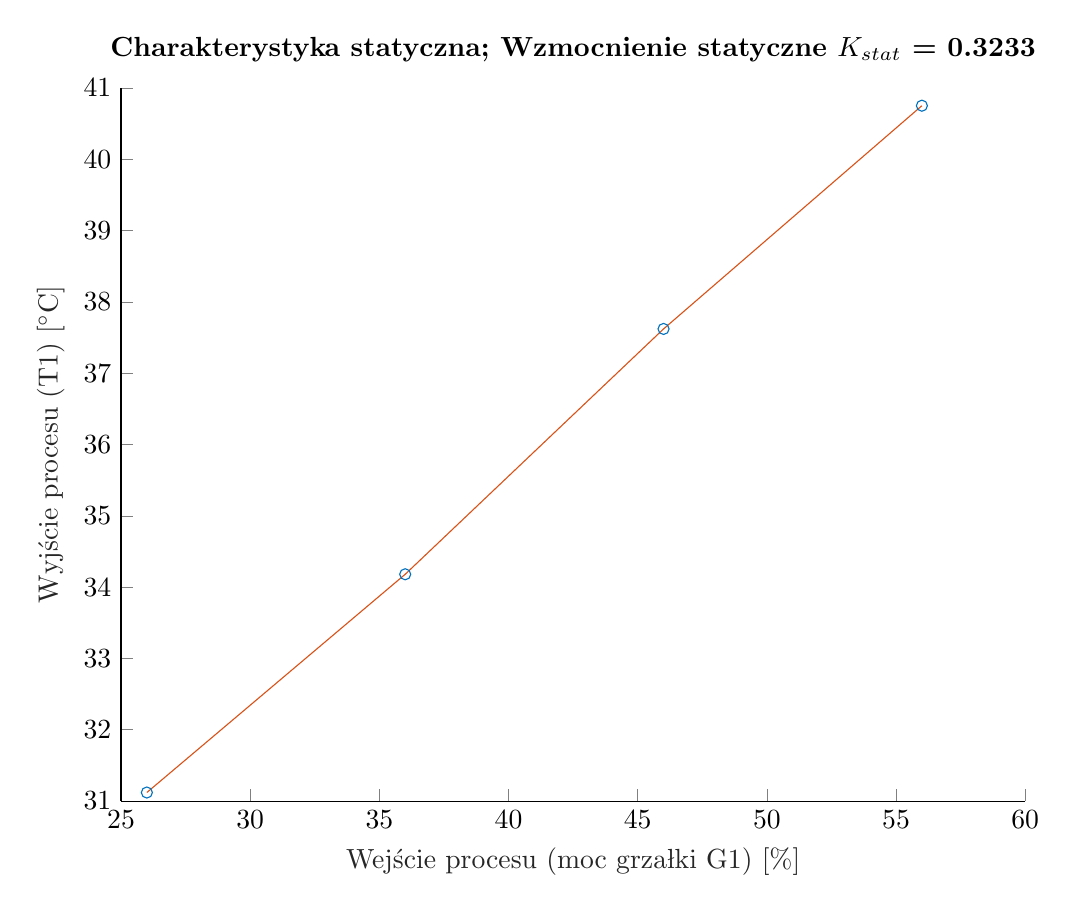
\begin{tikzpicture}

\begin{axis}[%
width=4.521in,
height=3.566in,
at={(0.758in,0.481in)},
scale only axis,
xmin=25,
xmax=60,
xlabel style={font=\color{white!15!black}},
xlabel={Wejście procesu (moc grzałki G1) [\%]},
ymin=31,
ymax=41,
ylabel style={font=\color{white!15!black}},
ylabel={Wyjście procesu (T1) [$^\circ$C]},
axis background/.style={fill=white},
title style={font=\bfseries},
title={Charakterystyka statyczna; Wzmocnienie statyczne $K_{stat}$ = 0.3233},
axis x line*=bottom,
axis y line*=left
]
\addplot [color=mycolor1, only marks, mark=o, mark options={solid, mycolor1}, forget plot]
  table[row sep=crcr]{%
26	31.12\\
36	34.18\\
46	37.62\\
56	40.75\\
};
\addplot [color=mycolor2, forget plot]
  table[row sep=crcr]{%
26	31.12\\
36	34.18\\
46	37.62\\
56	40.75\\
};
\end{axis}
\end{tikzpicture}%